\section{Background}
\label{sec:background}

\subsection{Total-Order Message Scattering}
\label{sec:toms}

\iffalse
\begin{figure}[t]
\centering
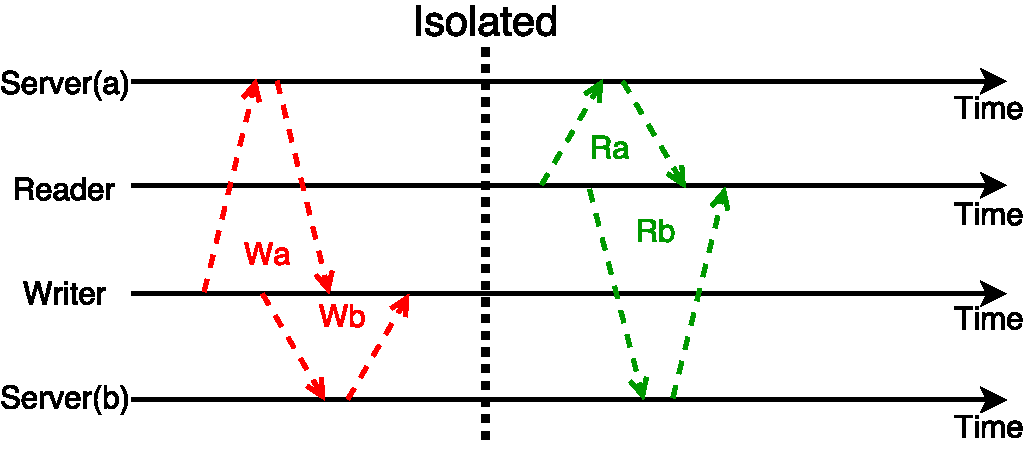
\includegraphics[width=0.48\textwidth]{images/read_write_isolation.pdf}
\caption{Two senders issue read and write requests to two receivers.}
\label{fig:example}
\end{figure}



\begin{figure}[t]
\centering
	\subfloat[Lock-based.\label{fig:concurrency-lock}]
	{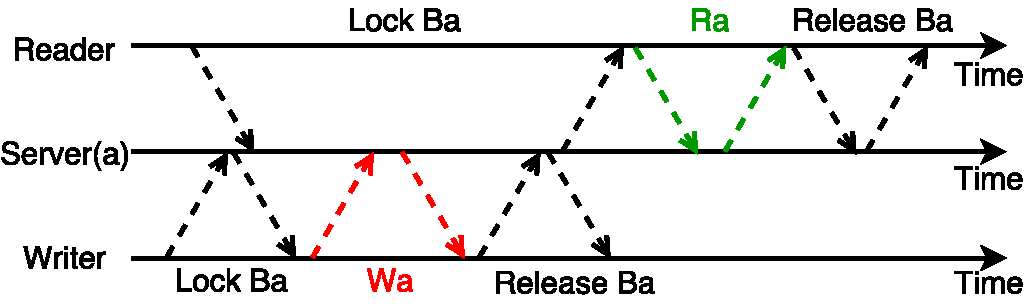
\includegraphics[width=.45\textwidth]{images/LockBased.pdf}}
    \hspace{0in}
	\subfloat[Timestamp-based (OCC).\label{fig:concurrency-timestamp}]
	{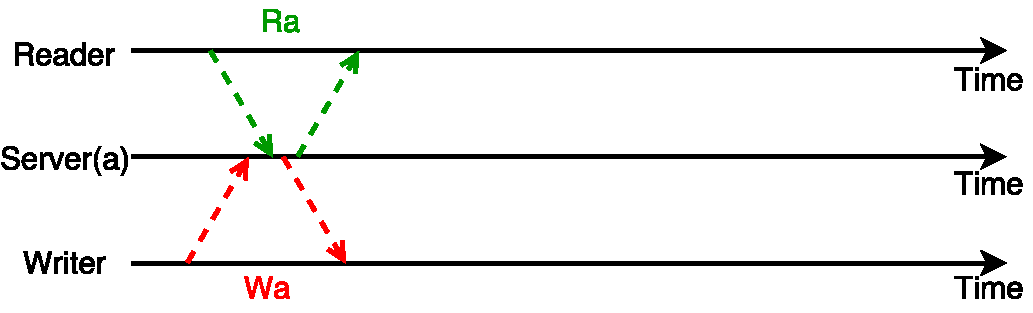
\includegraphics[width=.45\textwidth]{images/TimestampBased.pdf}}
	\caption{Two concurrency control mechanisms for distributed transactions.}
	\label{fig:concurrency-control}
\end{figure}
\fi


\begin{figure}[t]
\centering
	\subfloat[Possible causality violation due to variable network delay.\label{fig:causality_traditional}]
	{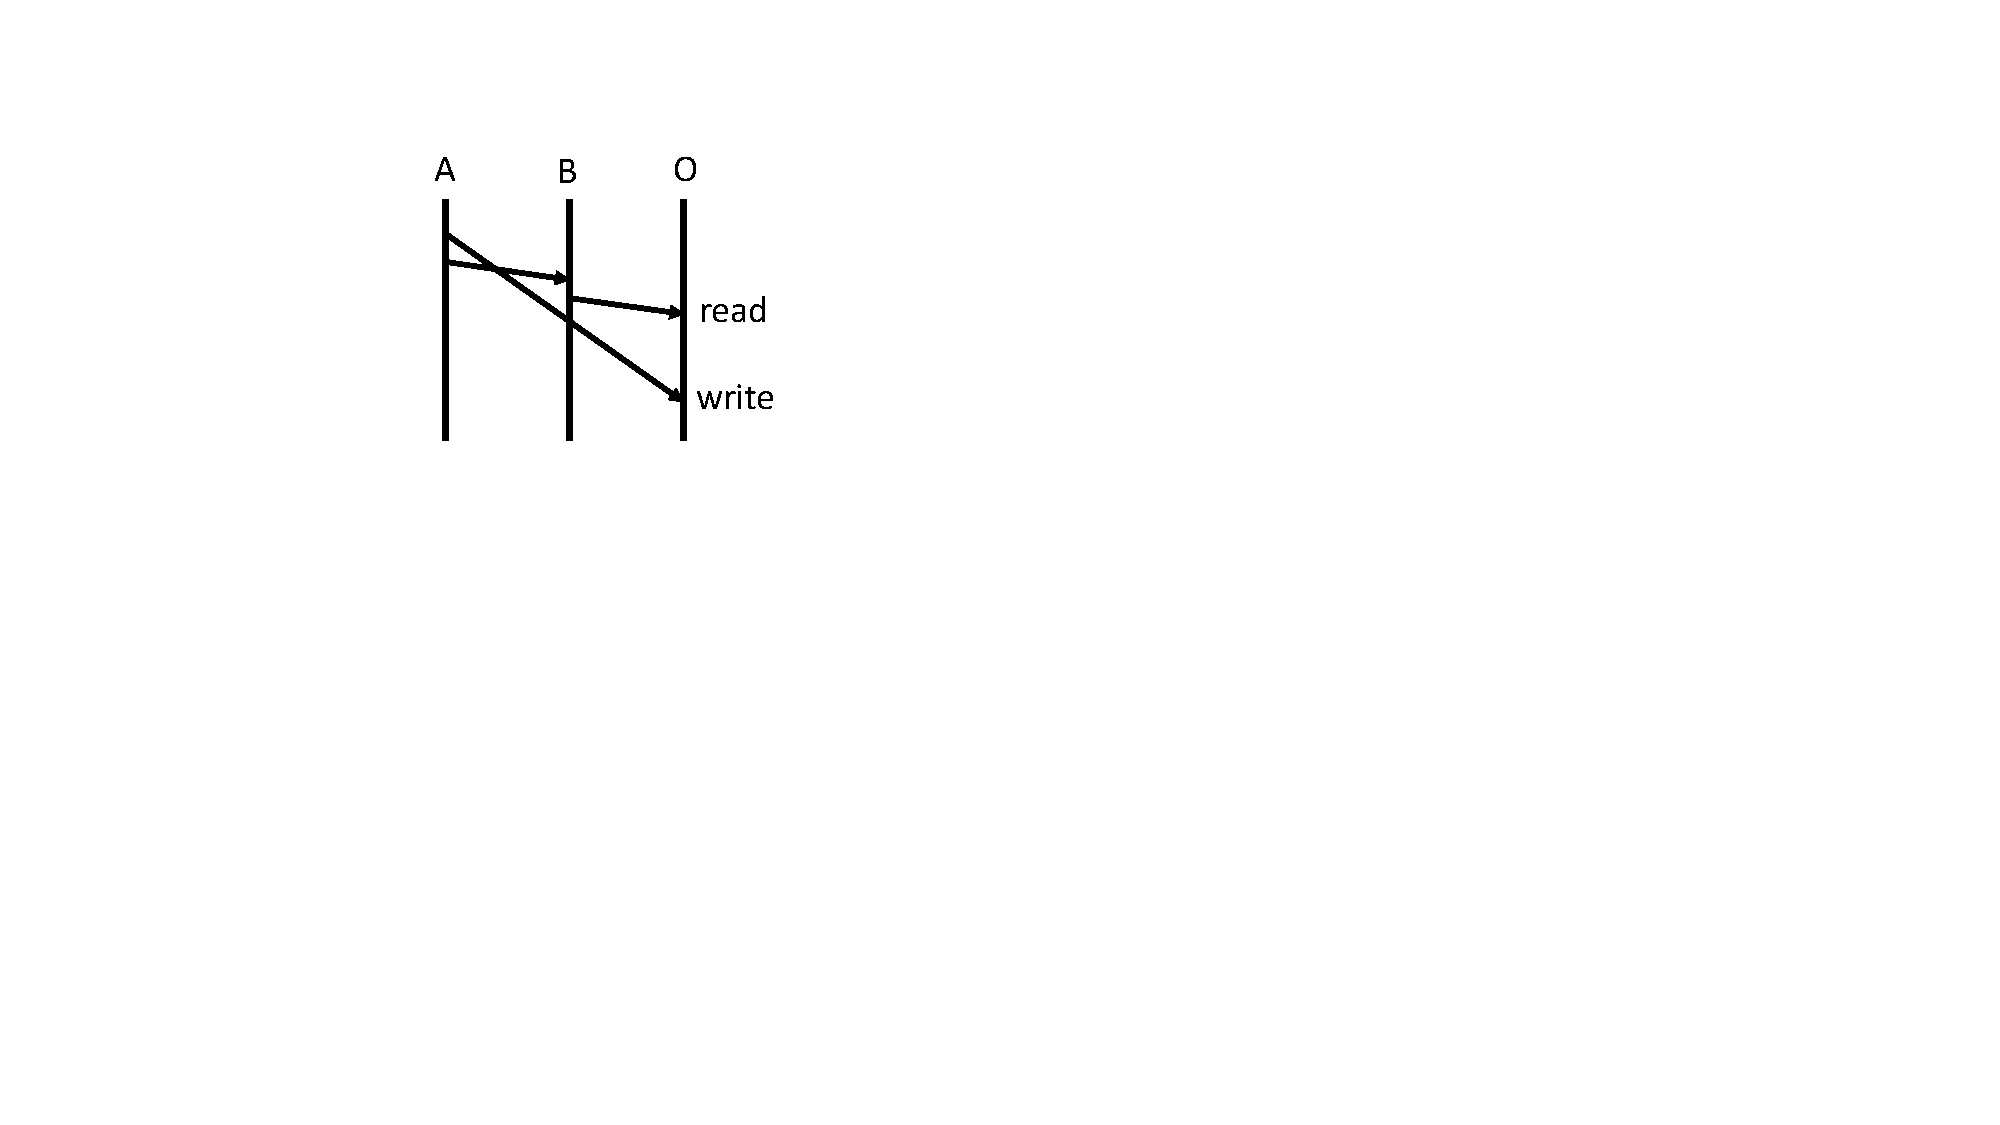
\includegraphics[width=.2\textwidth,page=1]{images/cropped_causality.pdf}}
    \hspace{0.03\textwidth}
	\subfloat[Guaranteed causality in \sys.]
	{\includegraphics[width=.2\textwidth,page=2]{images/cropped_causality.pdf}}
	\caption{Causality example: $A$ write shared object $O$, then notify $B$, then $B$ read $O$.}
	\label{fig:causality}
	\vspace{-1.5em}
\end{figure}


%The story begins with a hypothetical distributed banking system. Two accounts Alice and Bob are stored in different \textit{shards} at distant locations. Initially, their balances are $B_a$ and $B_b$. When Alice transfers \$1 to Bob, two write operations are sent to the shards: $B_a -= 1$ and $B_b += 1$, call them $W_a$ and $W_b$. At the same time, an auditor checks the total balance in the bank by accumulating balances of all accounts, resulting in two read operations: $R_a$ and $R_b$.
%If the system does not support transactions, the ordering of events may be $W_a < R_a < R_b < W_b$, then the auditor would find an inconsistent total balance.

In the distributed system, multiple \textit{hosts} are connected via the network. %A distributed system is made up of multiple \textit{hosts} connected via network. 
An \textit{event} occurs on a host, and scatters messages to other hosts. For example, a distributed single-round-trip transaction can be regarded as an event on the transaction initiator, and its read and write operations are sent to the shards where the objects are stored. Here we use the term \textit{scatter} instead of \textit{multicast} because each shard only needs to receive operations related to the objects it host.

We will use a hypothetical banking example to illustrate the main concepts. Two accounts Alice and Bob are stored in different \textit{shards} at distant locations. Initially, their balances are $B_a$ and $B_b$. When Alice transfers \$1 to Bob, two write operations are sent to the shards: $B_a -= 1$ and $B_b += 1$, call them $W_a$ and $W_b$. At the same time, an auditor checks the total balance in the bank by accumulating balances of all accounts, resulting in two read operations: $R_a$ and $R_b$. If the system does not support transactions, the ordering of events may be $W_a < R_a < R_b < W_b$, then the auditor would find an inconsistent total balance.

A strongly consistent distributed system requires the reads and writes to be \textit{transactional}. The transaction $R_a, R_b$ and the transaction $W_a, W_b$ need to be performed in isolation.

There are two main categories of concurrency control to implement a transactional system. One category uses \textit{locks} to protect accesses to shared resources. The read transaction needs to lock $B_a$ and $B_b$, and the write transaction also needs to lock them. The transaction throughput is bounded by the \textit{round-trip time} (RTT) between the clients and the shards, because the lock must be sent from the shard to the client, then the client may send unlock to the shard.
In our example scenario where all transactions need to lock a single resource, if the RTT is 100~$\mu$s, the throughput is bounded to 10K transactions per second.

The other category is \textit{optimistic concurrency control} (OCC). It assigns a \textit{timestamp} to each transaction ($T_R$ for read, $T_W$ for write) and tracks object accesses during transaction execution. Transactions are serialized according to timestamp order. Once the system detects a \textit{late write}, that is, the write operation has lower timestamp than a read operation ($T_W < T_R$) but arrives later ($R_a < W_a$ or $R_b < W_b$), one of the transactions needs to be aborted and retried with a higher timestamp.
%Due to variable delays between clients and shards, if the read and write transactions are initiated at almost the same time, there are many possible orderings of $R_a, R_b, W_a, W_b$ and $T_R, T_W$. 
If the network delays between clients and shards follow a normal distribution, for two conflicting concurrent transactions, the probability of aborting one transaction is 3/4 with two shards. If each transaction involves $N$ shards, the abort probability is $1-(\frac{1}{2})^N$.

%If we regard each transaction as an event on a client, then the \textit{event timestamp} is the transaction timestamp. The read and write operations are the effects of the events, which propagate to the shards via messages.
%Each event may \textit{scatter} a set of messages to receivers (shards in our example). Each message is tagged with the event timestamp. Different messages may be scattered to different receivers, so \textit{broadcast} is a special case of \textit{scatter}.

To implement OCC without transaction aborts, we propose \textit{total-order message scattering} (\sys). \sys assigns timestamps to events and scatters messages from events, so that each host delivers messages to applications in monotonically increasing timestamp order (break ties by sender ID).
\sys provides a total ordering of all events in a distributed system, and ensures that each node observes the events (via messages) consistent with the total ordering.
With \sys, we regard each single-round-trip transaction as an event on the transaction initiator. In the absence of failure, transaction abort in OCC will never be triggered, because the read and write operations are always received by shards in the same ordering according to transaction timestamps.

The application of \sys goes beyond distributed transactions. In a distributed shared memory system, if the remote memory accesses are transferred via \sys, then all remote memory accesses obey total store ordering, similar to x86 multi-core memory consistency model~\cite{sewell2010x86}. Improved memory consistency can greatly simplify distributed coordination in distributed shared memory~\cite{sewell2010x86}.
Figure~\ref{fig:causality} shows an example. $A$ first issues write to a shared object $O$, then sends a message to $B$. When $B$ receives the message, it issues read from $D$. Due to variable network delay, $B$ may read the old value of $O$, violating causality. In a traditional distributed system, $A$ must wait for the write operation to complete before notifying $B$, introducing additional delay. If all the messages are sent via \sys, the read operation is guaranteed to have a higher timestamp than the write operation, so $B$ is guaranteed to read the updated value of $O$.

It is worth noting that \sys ensures ordering instead of consensus. When some hosts experience failure, \sys does not ensure a quorum of hosts agree on its received messages. NOPaxos~\cite{li2016just} has shown that \sys leads to an efficient implementation of distributed consensus.

%In Sec.~\ref{sec:design}, we will return to this example to demonstrate how \sys works.

\subsection{Data Center Network}
\label{sec:dcn}


%\begin{figure*}[t]
%	\centering
%	\subfloat[Physical topology.\label{fig:dcn_tpo}]
%	{\includegraphics[width=.45\textwidth}{images/dcn_topology.pdf}}
%	\hspace{0.09\textwidth}
%	\subfloat[Expanded topology.\label{fig:dcn_dag}]
%	{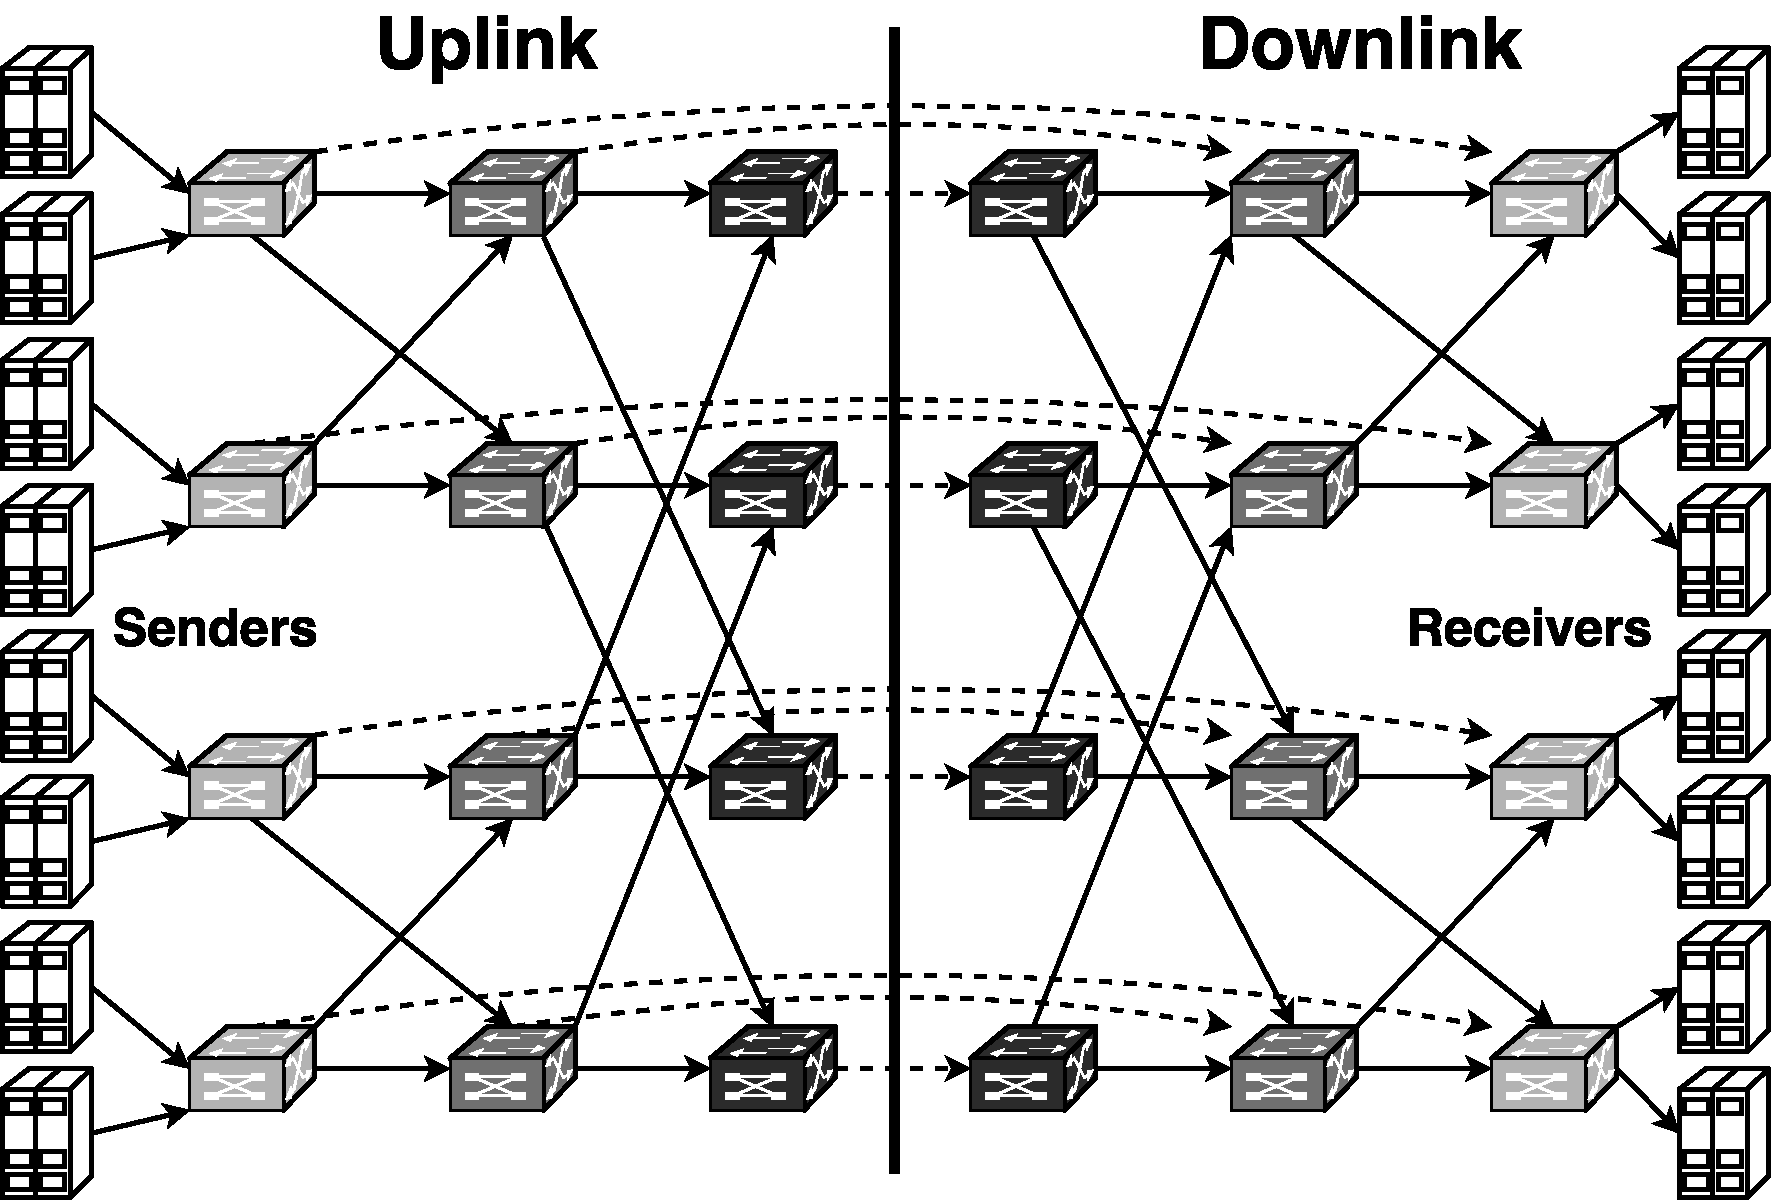
\includegraphics[width=.45\textwidth]{images/dcn_dag.pdf}}
%	\caption{Architecture of a typical data center network.}
%	\label{fig:dcn}
%\end{figure*}


\begin{figure}[t]
\centering
{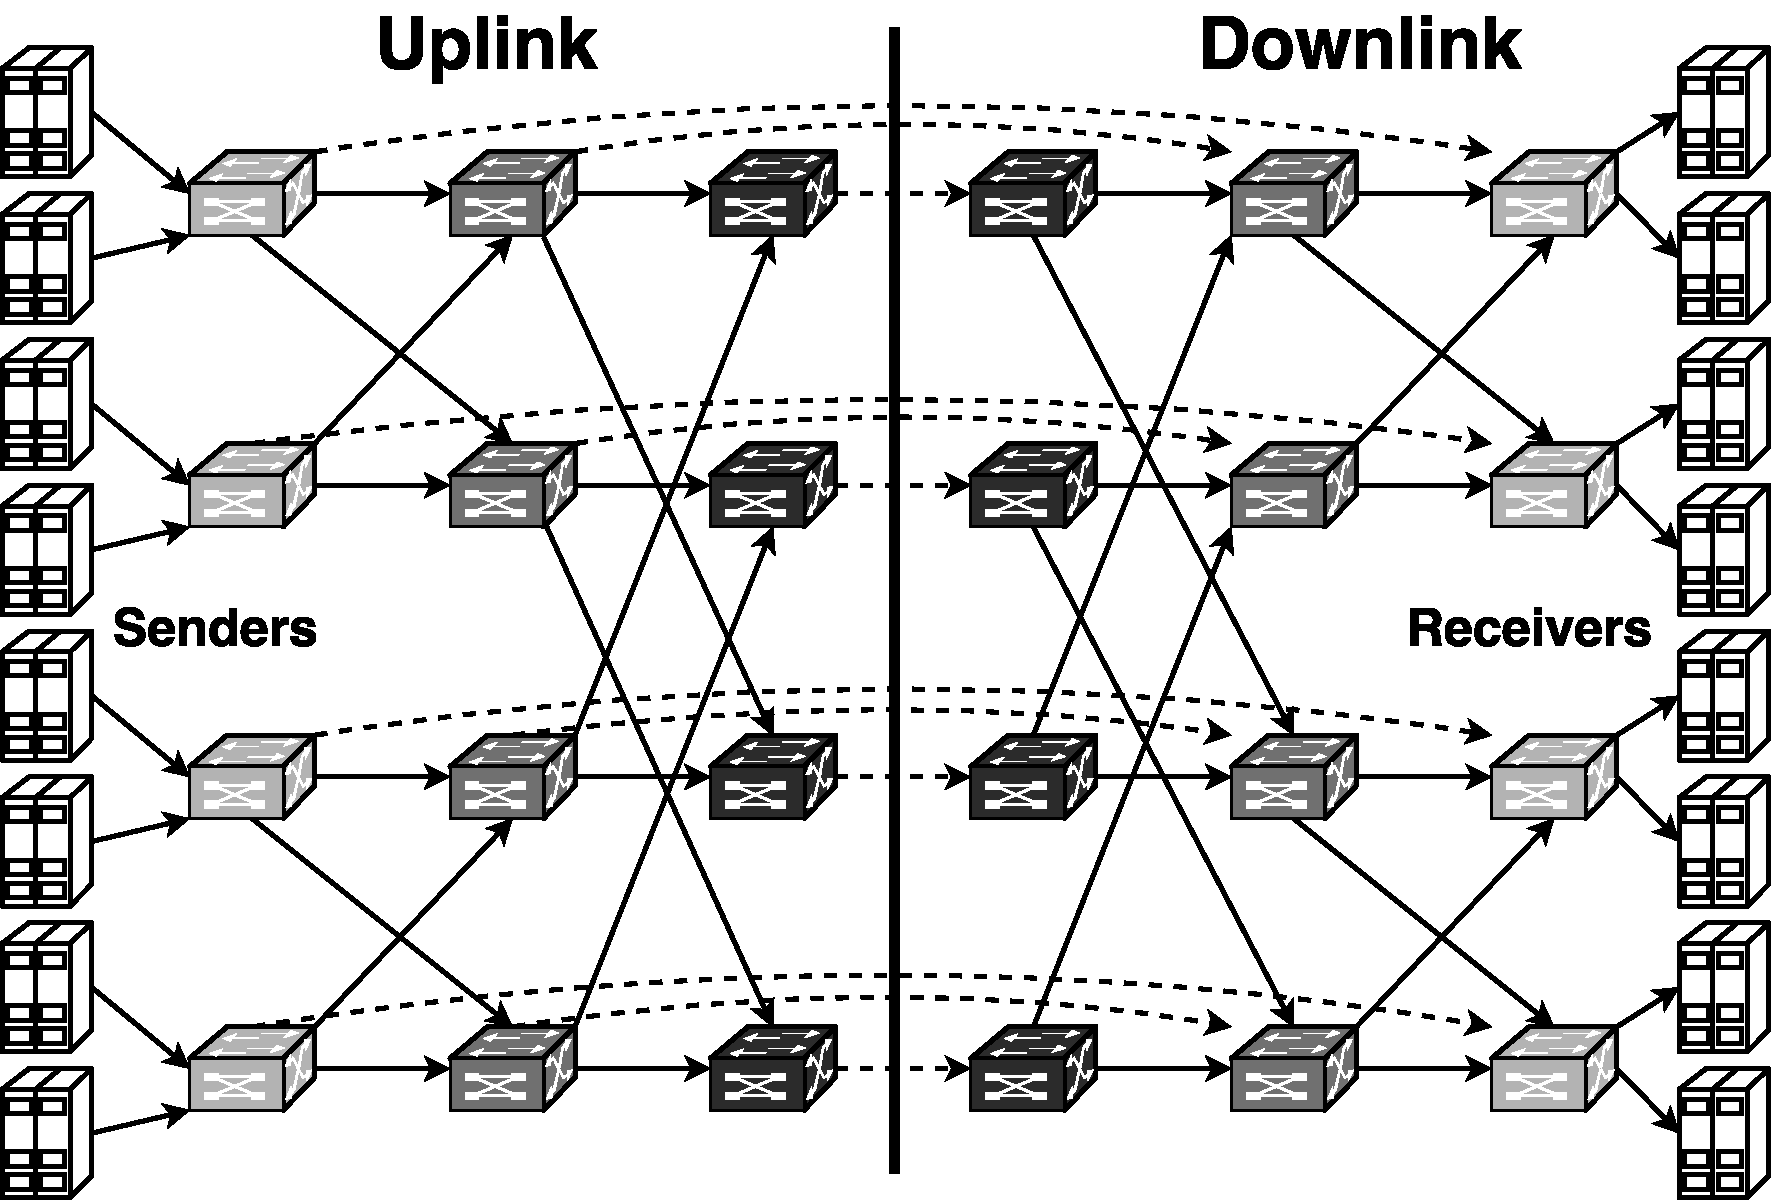
\includegraphics[width=.48\textwidth]{images/dcn_dag.pdf}}
\caption{Routing topology of a typical data center network. Each physical switch is split into two logical switches, one for uplink and one for downlink.}
\label{fig:dcn}
\vspace{-1.5em}
\end{figure}

\begin{figure}[t]
\centering
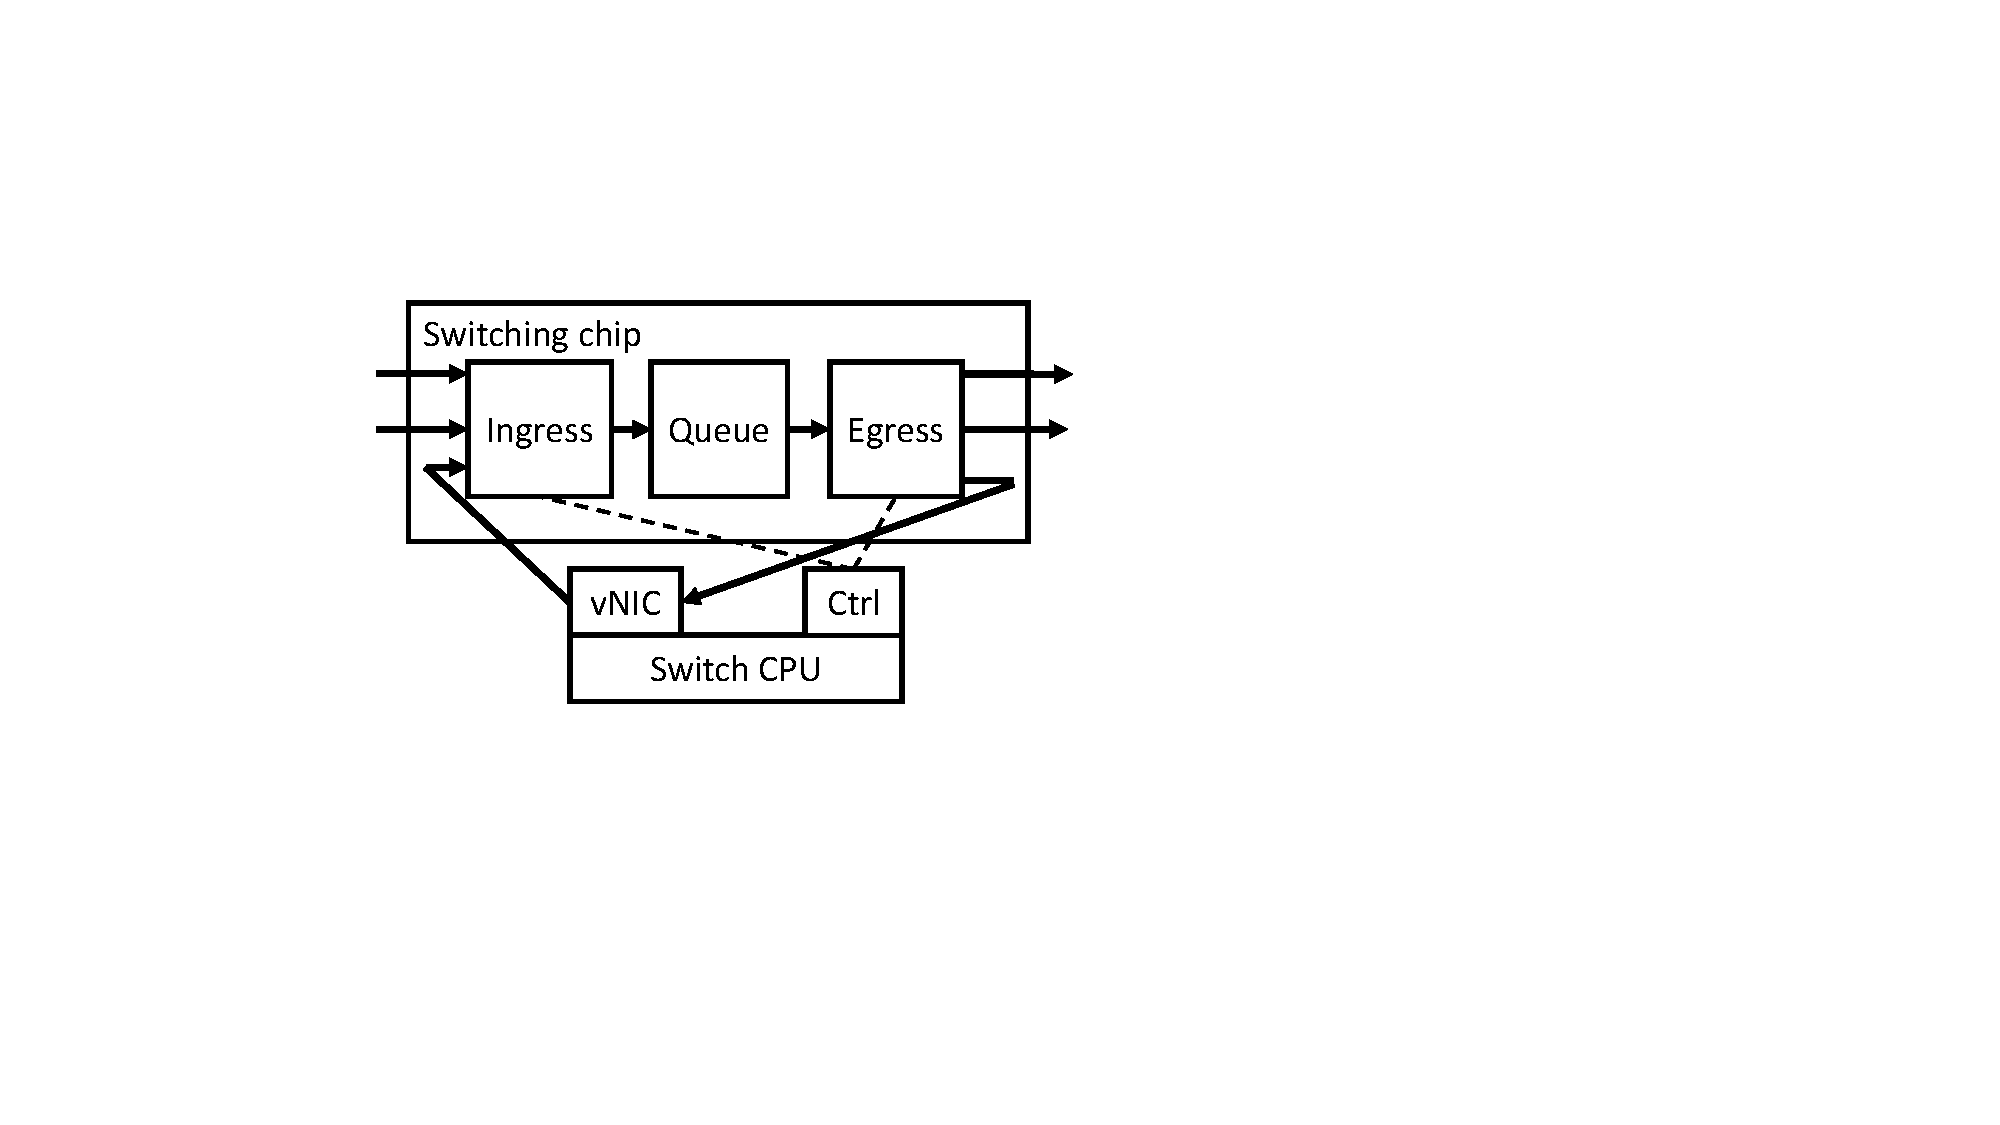
\includegraphics[width=0.3\textwidth]{images/cropped_switch_architecture.pdf}
\caption{Architecture of a typical network switch.}
\label{fig:switch}
\vspace{-1.5em}
\end{figure}

Moderen data centers typically adopt multi-rooted tree topologies~\cite{leiserson1985fat,greenberg2009vl2} to interconnect hundreds of thousands of end hosts. Shortest-path routing between two servers in a fat-tree first goes up layers of switches to one of their common ancestors, then goes down layers of switches. Therefore, the routing topology form a directed acyclic graph (DAG), as shown in Figure~\ref{fig:dcn}.  

%In a modern data center, servers (\textit{end hosts}) are typically organized as the leaves of a fat-tree, while the \textit{network switches} form multiple layers of internal nodes. Shortest-path routing between two servers in a fat-tree first goes up layers of switches to one of their common ancestors, then goes down layers of switches. Therefore, the routing topology form a directed acyclic graph (DAG), as shown in Figure~\ref{fig:dcn}.

The typical data center switch consists of a switching chip~\cite{broadcom} and a CPU (Figure~\ref{fig:switch}). The switch operating system~\cite{arista-eos} software running on the CPU controls the switching chip (\textit{e.g.} configure chip register values). The switching chip can transfer traffic (typically control plane packets, such as DHCP and BGP) to CPU via a virtual NIC.

The data center switch can provide good programmability. First, the CPU can be used to co-process (a small amount of) data plane packets with high flexibility\cite{lu2011serverswitch}. Second, the switching chip is becoming more and more programmable in recent years. For example, Tofino chip from Barefoot networks~\cite{tofino} uses RMT architecture~\cite{bosshart2013forwarding} with flexiable packet parsers and reconfigurable match action table pipelines. It can be programmed using P4~\cite{bosshart2014p4} to achieve \textit{flexible per-packet processing}.   

However, despite the good programmability, the data center switch typically has the limited buffer resource for low cost. The average per-port on-chip buffer size is typically hundreds of KB~\cite{bai2017congestion}. Furthermore, the buffer size per port per Gbps keeps decreasing with the increase of the link speed. As a result, 
it is very challenging to buffer many packets at the data center switch.
 
%, controls the switching chip and communicates with other switches via a management network. 

%There is a CPU port on the switching chip and a virtual NIC on the CPU to transfer control-plane packets (\textit{e.g.} DHCP, BGP) between the chip and the CPU. 


%Logically, the switching chip is composed of an \textit{ingress} pipeline, multiple queues and an \textit{egress} pipeline.
%Both ingress and egress pipelines are a chain of match-action tables. Each table can accomodate a number of rules. Each rule matches a set of packet header fields and internal states, and applies a limited repertoire of actions corresponding to common processing behaviors.
%When a packet is received from an ingress link, it first goes through the ingress pipeline (including tunnel decapsulation, routing, ACL rules and others) to determine the egress port and queueing priority, then get buffered into the tail of the queue of corresponding priority. The egress pipeline pulls packets from the head of each queue according to scheduling disciplines, applies header modifications and sends them to the egress links. This queueing model ensures FIFO property for packets with same priority.

%One limitation of most widely-deployed switching chips is the limited programmability of internal states that are persistent across packets. The Barefoot Tofino switching chip~\cite{tofino} using RMT architecture~\cite{bosshart2013forwarding} supports \textit{stateful per-packet processing} and has high programmability with P4~\cite{bosshart2014p4} language.
%However, the number of persistent states supported by each switch is only sufficient to have several per-port registers, but not enough to maintain per-packet states. 
%Furthermore, the buffer size of network switches is less than 1~MB per port~\cite{bai2017congestion}.
%Therefore, it is hard to implement a strict priority queue large enough for in-network serialization~\cite{sivaraman2016programmable}.

%\subsection{In-Network Computation}
%\label{sec:in-network}

%In-network computation flourishes with the trend of programmable switches (cite P4, Domino, serverswitch) and NICs (cite ClickNP, flexnic, VFP), opening up two categories of opportunities to distributed systems:

%\textit{Increase knowledge and control in network transmission.}
%In modern datacenters, there are multiple paths from a sender to a receiver for load balancing and fault tolerance. 
%Software-defined networking (SDN) enables visibility to routing table changes from BGP or administrators. In our scenario, in order to know the set of all possible ingress ports per egress port, \sys software on the affected switches need to be notified prior to route change.

%\textit{Offload computation on end hosts to reduce network traffic and latency.}
%\textit{Multicast} is an in-network computation to reduce duplication of messages on sender side.
%\textit{On-switch cache} is also a type of in-network computation to save computation on end hosts and improve load balancing (cite switchKV).
%A single network switch is a serialization point where \textit{coordination} of directly-connected hosts can take place (cite hardware coordination, Eris).
%\sys leverages the broadcast, cache and coordination functionalities of network switches to scale total ordering hierarchically.\RED{(leverage broadcast and cache?)}

\subsection{Design Goals}
\label{sec:goals}

Our goal is to build a scalable total-order message scattering service on top of existing network infrastructure in geographically distributed data centers. Such a service should satisfy the following requirements.

\textbf{Scalable.}
Eris~\cite{eris} proposed an efficient solution for total-order broadcast using centralized sequencers. However, for large-scale deployments, the throughput of the centralized sequencer would become bottleneck. In our proposal, the system is decentralized.
Additionally, for ease of deployment, it is also highly desirable for the algorithms running on each end host or network switch to be logically equivalent.

\textbf{Efficient.}
The reordering delay between end host receiving the message and delivering the message to application should be minimal. This requires senders to assign timestamps properly so that messages with similar timestamps arrive at receivers as synchronized as possible. Furthermore, the network and computation overhead of total ordering should be minimal.


%\textbf{Low Network Bandwidth Overhead.}
%Additional packets generated for ensuring ordering should be minimal. The metadata tagged on each packet should also be minimal.

%\textbf{Low CPU Overhead.}
%Because the CPUs on switches are typically not very powerful, the processing on switch CPU should be as simple and infrequent as possible. Moreover, the reordering overhead on end hosts should also be reasonable.

\textbf{Fault-Tolerant.}
The correctness of the system should not be violated under packet loss, or failure of one or more switches, links or end hosts.


\textbf{Readily Deployable.}
The service should be readily deployable using existing commodity switching hardware in data centers.

%\textbf{Adaptive to Delay Variance.}
%The delay among geographically distributed datacenters can be hundreds of milliseconds.
%Because commodity NIC hardware is not able to assign a same timestamp to a group of scattered messages, \sys assigns timestamps in software.
%Different OS network stacks have more than 100~$\mu$s of processing delay differences, and it may grow to milliseconds under heavy load.
%Links with different speeds or congestions also lead to delay variations.
%The system should dynamically adapt to the variance of network delays to minimize reordering delay.

\subsection{Network Requirements}
\label{sec:assumptions}

\sys assumes that the underlying network satisfies three properties, two for correctness and one for liveness.

\textbf{At-most-once transport.}
The underlying transport of \sys should provide at-most-once semantics, \textit{i.e.}, each packet is transmitted at most once. Otherwise, the retransmitted packet may violate timestamp ordering on the network link. UDP/IP or unreliable datagram in RDMA satisfies this requirement.

\textbf{FIFO on a Network Switch.}
If packets $P_1, P_2$ arrive in order to an ingress port of switch $S$, and they are routed to the same egress port, then their egress ordering should also be $P_1, P_2$. In practice, packets from the same application typically have the same priority, so packet ordering is preserved after passing through a single switch.

\textbf{Loop-Free Routing.}
%Formally, for a switch $S$, its egress ports $E$ and ingress ports $I$, if there is a possible route from an ingress port $i \in I$ to an egress port $e \in E$, then add $i$ to the \textit{ingress set} of $e$.
Formally, for $n$ distinct switches $S_1, \ldots, S_n$, if there are $n$ links $L_1, \ldots, L_n$ directly connecting $S_1 \rightarrow S_2, \ldots, S_{n-1} \rightarrow S_n, S_n \rightarrow S_1$, and $n$ possible routes (need not be distinct) passing through $L_1 \rightarrow L_2, \ldots, L_{n-1} \rightarrow L_n, L_n \rightarrow L_1$ respectively, then we call it a \textit{routing loop}. Loop-free is a liveness requirement. A routing loop stalls the update of timestamp barriers, but does not violate correctness.
%Sec.~\ref{sec:eval-changes} evaluates temporary routing loops.
%Shortest-path (ECMP) routing in a Clos network is loop-free, which is common in datacenters.
%Shortest-path routing in a triangle is also loop-free. However, shortest-path routing in a pentagon is not loop-free, because the 5 routes $S_1 \rightarrow S_2 \rightarrow S_3, \ldots, S_5 \rightarrow S_1 \rightarrow S_2$ form a routing loop by our definition.
